\documentclass{article}

\usepackage[utf8]{inputenc}
\usepackage{mdwlist}
\usepackage[inner=3cm,outer=4cm]{geometry}
\usepackage{mathtools}

\usepackage{Sweave}
\begin{document}
\Sconcordance{concordance:HW09MANOVA_DA.tex:HW09MANOVA_DA.Rnw:%
1 7 1 1 0 27 1 1 2 1 0 4 1 1 2 7 1 3 0 2 2 1 0 1 2 1 0 1 2 1 0 1 2 1 0 %
1 3 9 0 1 2 7 1 1 4 3 0 1 1 16 0 1 1 4 0 1 2 5 1 1 2 1 0 2 1 134 0 1 1 %
13 0 1 1 1 2 6 0 2 1 1 2 10 0 1 2 6 1 1 3 2 0 1 1 10 0 1 2 15 1 1 2 1 0 %
5 1 65 0 1 2 6 1 1 2 1 0 1 1 7 0 1 2 6 1 1 2 1 0 2 1 25 0 1 1 14 0 3 1 %
1 5 3 0 1 1 14 0 1 2 6 1 1 2 9 0 1 2 12 1}


\title{Homework 09. Discriminant Analysis and MANOVA. PLS206 Fall 2014}
\author{Emilio A. Laca and Matt Espe}
\maketitle


\section {Discriminant Analysis}
\subsection{Instructions}
Use the file seedDA.txt. These are data on the dimensions of seeds from three species, \emph{Bromus hordeaceous}, \emph{Bromus madritensis} and \emph{Lolium multiflorum}. It is known that there are no other seeds in the mixtures. Exclude the rows where hold.out=1 and develop a discriminant rule based on all morphological variables with the remaining rows.

\begin{description*}
  \item[spp] species of seed.
  \item[area] area of seed projection ("shadow").
  \item[perimeter] perimeter of seed projection mm.
  \item[length] seed length mm.
  \item[width] seed width mm.
  \item[area.per] area:perimeter ratio.
  \item[len.wid] length:width ratio.
  \item[hold.out] 1 = hold.out sample, 0 = training sample.
\end{description*}


\subsection{Homogeneity of variance [10]}
Determine if there is heterogeneity of variance covariance by using a couple of 3D plots. Report the plots using a couple of suitable perspectives.

The first chunk of code loads the necessary packages, read the data and adds residuals to the data file.
\begin{Schunk}
\begin{Sinput}
> library(MASS)
> library(rgl)
> library(klaR)
> library(candisc)
> library(rpart)
> seeds <- read.csv("../Examples/seedDA.txt", header=TRUE)
> tseeds <- split(seeds, seeds$hold.out)[[1]]
> vseeds <- split(seeds, seeds$hold.out)[[2]]
> mvres <- as.data.frame(residuals(manova(cbind(area,perimeter,length,width,area.per,len.wid) ~ spp, tseeds)))
> names(mvres) <- paste(names(mvres),".r", sep="")
> tseeds <- cbind(tseeds, mvres)
> colors <- c("blue", "green", "orange")
> tseeds$color <- factor(tseeds$spp, labels = colors)
\end{Sinput}
\end{Schunk}

\begin{Schunk}
\begin{Sinput}
> tseeds.by.spp <- split(tseeds, tseeds$spp)
> # calculate covariances for ellipses
> tseeds.cov <- lapply(tseeds.by.spp, function(x) cov(x[,c(11,12,14)]))
>  # calculate centroids for ellipses
> tseeds.means <- lapply(tseeds.by.spp, function(x) colMeans(x[,c(4,5,7)]))
> # plot residuals
> with(tseeds, plot3d(length.r, width.r, len.wid.r,  type = "s", col = color, size = 1))
> # add ellipses to residuals
> sapply(seq_along(tseeds.cov), function(i) plot3d(ellipse3d(tseeds.cov[[i]]), 
+        col = colors[i], alpha = 0.4, add = TRUE))
\end{Sinput}
\begin{Soutput}
quads quads quads 
   11    12    13 
\end{Soutput}
\end{Schunk}

The 3D plots show that the green hyperellipsoid for \emph{B. adritensis} is larger than and has orientation different from the other two specie. Therefore, a quadratic discriminant function may work better than the linear one.

\subsection{Discriminant analysis [10]}

Use a linear or quadratic discriminant function according to your assessment. Set prior probabilities to be equal.
We use a quadratic discriminant. Once the discriminant is calculated we can display the regions for classification in a graphical form. We use partition plots from the \verb!klaR! package.

\begin{Schunk}
\begin{Sinput}
> qseeds <- qda(x = tseeds[,2:7], 
+               grouping = tseeds$spp,
+               prior = c(1, 1, 1) / 3)
> qseeds
\end{Sinput}
\begin{Soutput}
Call:
qda(tseeds[, 2:7], grouping = tseeds$spp, prior = c(1, 1, 1)/3)

Prior probabilities of groups:
     brho      brma      lomu 
0.3333333 0.3333333 0.3333333 

Group means:
         area perimeter    length    width  area.per  len.wid
brho 10.99422  16.45457  6.909055 2.011132 0.6623946 3.493304
brma 13.53324  24.93078 10.810935 1.593234 0.5471097 6.918747
lomu  9.35853  13.98133  5.650880 2.084783 0.6607192 2.750462
\end{Soutput}
\begin{Sinput}
> partimat(spp ~ area+perimeter+length+width+area.per+len.wid, tseeds, method="qda")
\end{Sinput}
\end{Schunk}
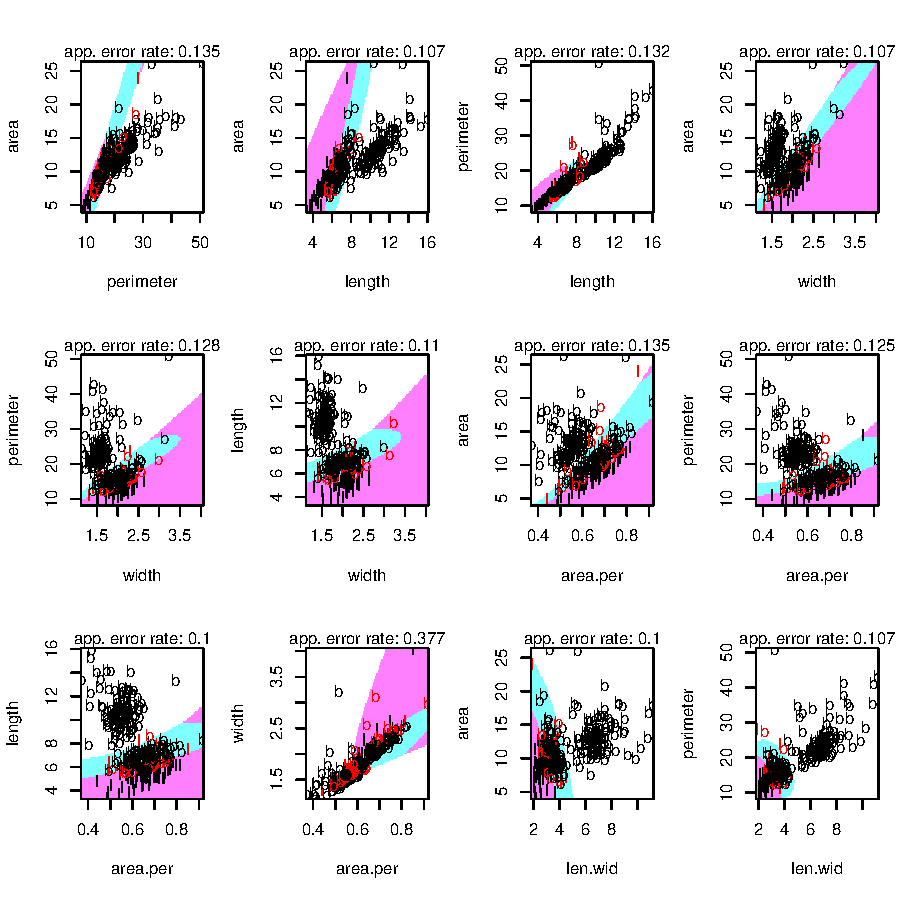
\includegraphics{HW09MANOVA_DA-003}

\subsection{Canonical plots and loadings [10]}
Report the discriminant plot using the first two canonical variables and indicate what original variables are related to canonical 1 and 2 by using the correlations (loadings) with the original variables.

For this part we need to use the linear discriminant for simplicity. Canonical variates are not easiluy defined or calculated in quadratic discriminant analysis.

\begin{Schunk}
\begin{Sinput}
> library(candisc)
> mvmod <- lm(cbind(area,perimeter,length,width,area.per,len.wid) ~ spp, tseeds)
> summary(mvmod)
\end{Sinput}
\begin{Soutput}
Response area :

Call:
lm(formula = area ~ spp, data = tseeds)

Residuals:
    Min      1Q  Median      3Q     Max 
-6.7572 -1.9062 -0.1852  1.2595 14.6555 

Coefficients:
            Estimate Std. Error t value Pr(>|t|)    
(Intercept)  10.9942     0.2890  38.037  < 2e-16 ***
sppbrma       2.5390     0.3932   6.458 4.73e-10 ***
spplomu      -1.6357     0.4185  -3.909 0.000117 ***
---
Signif. codes:  0 ‘***’ 0.001 ‘**’ 0.01 ‘*’ 0.05 ‘.’ 0.1 ‘ ’ 1

Residual standard error: 2.757 on 278 degrees of freedom
Multiple R-squared:  0.2859,	Adjusted R-squared:  0.2808 
F-statistic: 55.65 on 2 and 278 DF,  p-value: < 2.2e-16


Response perimeter :

Call:
lm(formula = perimeter ~ spp, data = tseeds)

Residuals:
     Min       1Q   Median       3Q      Max 
-11.6078  -2.1476  -0.5248   1.0087  26.0652 

Coefficients:
            Estimate Std. Error t value Pr(>|t|)    
(Intercept)  16.4546     0.4333  37.972  < 2e-16 ***
sppbrma       8.4762     0.5895  14.379  < 2e-16 ***
spplomu      -2.4732     0.6274  -3.942 0.000102 ***
---
Signif. codes:  0 ‘***’ 0.001 ‘**’ 0.01 ‘*’ 0.05 ‘.’ 0.1 ‘ ’ 1

Residual standard error: 4.134 on 278 degrees of freedom
Multiple R-squared:  0.5756,	Adjusted R-squared:  0.5726 
F-statistic: 188.5 on 2 and 278 DF,  p-value: < 2.2e-16


Response length :

Call:
lm(formula = length ~ spp, data = tseeds)

Residuals:
    Min      1Q  Median      3Q     Max 
-4.9279 -0.6219 -0.0061  0.4701  5.2091 

Coefficients:
            Estimate Std. Error t value Pr(>|t|)    
(Intercept)   6.9091     0.1239  55.755  < 2e-16 ***
sppbrma       3.9019     0.1686  23.147  < 2e-16 ***
spplomu      -1.2582     0.1794  -7.012 1.78e-11 ***
---
Signif. codes:  0 ‘***’ 0.001 ‘**’ 0.01 ‘*’ 0.05 ‘.’ 0.1 ‘ ’ 1

Residual standard error: 1.182 on 278 degrees of freedom
Multiple R-squared:  0.7842,	Adjusted R-squared:  0.7826 
F-statistic: 505.1 on 2 and 278 DF,  p-value: < 2.2e-16


Response width :

Call:
lm(formula = width ~ spp, data = tseeds)

Residuals:
     Min       1Q   Median       3Q      Max 
-0.77578 -0.17923 -0.01578  0.12787  1.95822 

Coefficients:
            Estimate Std. Error t value Pr(>|t|)    
(Intercept)  2.01113    0.03227  62.313   <2e-16 ***
sppbrma     -0.41790    0.04390  -9.518   <2e-16 ***
spplomu      0.07365    0.04673   1.576    0.116    
---
Signif. codes:  0 ‘***’ 0.001 ‘**’ 0.01 ‘*’ 0.05 ‘.’ 0.1 ‘ ’ 1

Residual standard error: 0.3079 on 278 degrees of freedom
Multiple R-squared:  0.3442,	Adjusted R-squared:  0.3395 
F-statistic: 72.97 on 2 and 278 DF,  p-value: < 2.2e-16


Response area.per :

Call:
lm(formula = area.per ~ spp, data = tseeds)

Residuals:
      Min        1Q    Median        3Q       Max 
-0.222180 -0.044400  0.004026  0.043699  0.254604 

Coefficients:
             Estimate Std. Error t value Pr(>|t|)    
(Intercept)  0.662395   0.007709   85.93   <2e-16 ***
sppbrma     -0.115285   0.010486  -10.99   <2e-16 ***
spplomu     -0.001675   0.011161   -0.15    0.881    
---
Signif. codes:  0 ‘***’ 0.001 ‘**’ 0.01 ‘*’ 0.05 ‘.’ 0.1 ‘ ’ 1

Residual standard error: 0.07353 on 278 degrees of freedom
Multiple R-squared:  0.3662,	Adjusted R-squared:  0.3616 
F-statistic: 80.31 on 2 and 278 DF,  p-value: < 2.2e-16


Response len.wid :

Call:
lm(formula = len.wid ~ spp, data = tseeds)

Residuals:
    Min      1Q  Median      3Q     Max 
-3.7054 -0.4458 -0.0317  0.3616  4.2606 

Coefficients:
            Estimate Std. Error t value Pr(>|t|)    
(Intercept)  3.49330    0.09766  35.768  < 2e-16 ***
sppbrma      3.42544    0.13286  25.783  < 2e-16 ***
spplomu     -0.74284    0.14141  -5.253 2.98e-07 ***
---
Signif. codes:  0 ‘***’ 0.001 ‘**’ 0.01 ‘*’ 0.05 ‘.’ 0.1 ‘ ’ 1

Residual standard error: 0.9317 on 278 degrees of freedom
Multiple R-squared:  0.8009,	Adjusted R-squared:  0.7994 
F-statistic: 559.1 on 2 and 278 DF,  p-value: < 2.2e-16
\end{Soutput}
\begin{Sinput}
> mvmod
\end{Sinput}
\begin{Soutput}
Call:
lm(formula = cbind(area, perimeter, length, width, area.per, 
    len.wid) ~ spp, data = tseeds)

Coefficients:
             area       perimeter  length     width      area.per   len.wid  
(Intercept)  10.994220  16.454571   6.909055   2.011132   0.662395   3.493304
sppbrma       2.539023   8.476204   3.901880  -0.417898  -0.115285   3.425443
spplomu      -1.635690  -2.473246  -1.258175   0.073651  -0.001675  -0.742842
\end{Soutput}
\begin{Sinput}
> cd.mvmod <- candisc(mvmod)
> # biplot ob observations and canonical variates
> plot(cd.mvmod)
\end{Sinput}
\begin{Soutput}
Vector scale factor set to  8 
\end{Soutput}
\begin{Sinput}
> can1 <- cd.mvmod$scores$Can1
> can2 <- cd.mvmod$scores$Can2
> # extract canonical variables from candisc object
> cor(cbind(can1,can2),tseeds[,2:7])
\end{Sinput}
\begin{Soutput}
           area   perimeter      length      width   area.per    len.wid
can1 -0.5711984 -0.82208813 -0.95950773  0.6337101  0.6394720 -0.9683343
can2 -0.2320487  0.01344257 -0.02569905 -0.1221446 -0.3469659  0.1240320
\end{Soutput}
\end{Schunk}
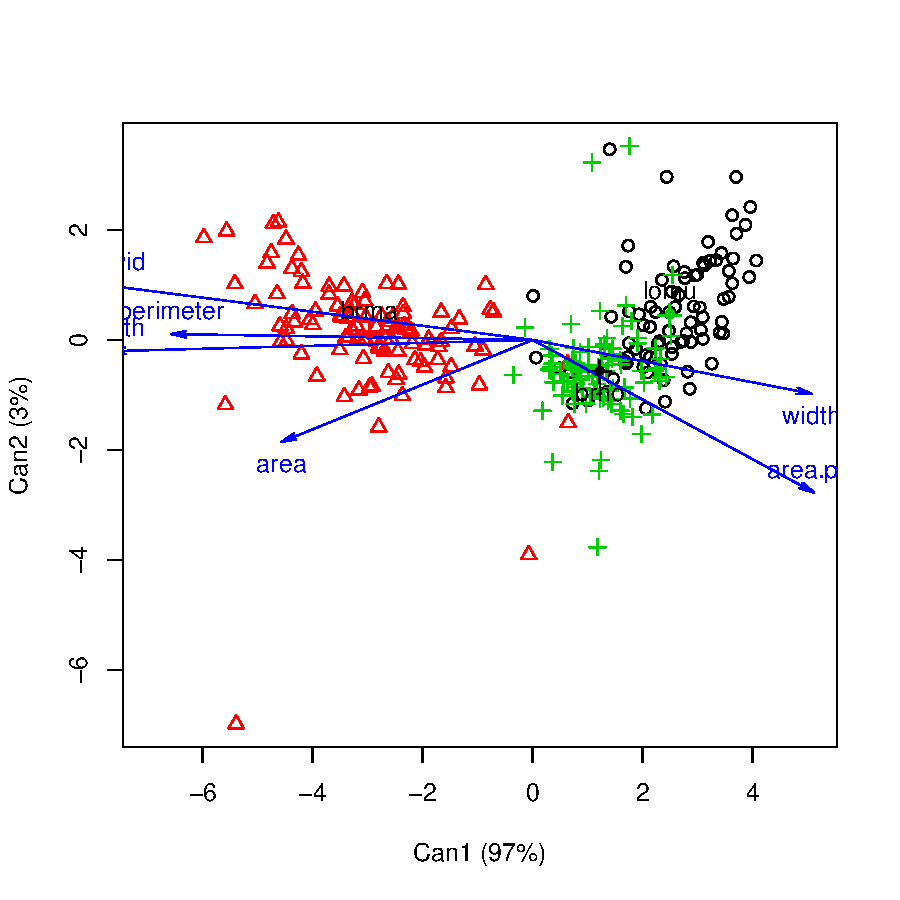
\includegraphics{HW09MANOVA_DA-004}

The canonical plot shows that most of the differences are between brma and the other two species. Brma tended to have longer and narrower seeds than brho and lomu. Lomu and brho difered mainly in area. The first canonical variable was higly correlated with length and length: width ration, whereas the second canonical variable was negatively correlated with area:perimeter ratio and area.

\subsection{Error rate [10]}

Estimate the error rate using the data held out with the same method used in the iris example.

\begin{Schunk}
\begin{Sinput}
> qd.pred <- predict(qseeds, newdata = vseeds[,2:7],
+                     method = "debiased", prior = c(1/3,1/3,1/3))
> xtabs(~ vseeds$spp + qd.pred$class)
\end{Sinput}
\begin{Soutput}
          qd.pred$class
vseeds$spp brho brma lomu
      brho   13    0    8
      brma    0   17    0
      lomu    3    0    9
\end{Soutput}
\end{Schunk}

The probability of error depends on the true species. For example, no errors are made when the true seeds is brma, but some brho and lomu are misclassified. Thus, the relative proportions of the species in the population being classified affects the effective error rate. Assuming seeds are present in equal proportions, overall the error rate is (0.333*7 + 0.333*3)/50.

\subsection{Prior probabilities. [10]}
What is a prior probability? Explain it in your words. You can use an example.

The prior probabilities for a classification problem are the probabilities of randomly obtaining objects of each class. For example, the prior for brho would be the probability of ontaining a brho seed. If the seed is obtained at random from the population of seeds, it is reasonable to assume that the probability is proportional to the relative abundance of the seed.

\section{MANOVA}

A study was conducted to determine if plants of a species (from seeds collected in different regions) show evidence of adaptation. Seeds of Phytus imaginarius were collected both at a variety of sites in the Great Basin deserts and in many sites in the intermediate elevations of the Sierra Nevada (ecotypes). A random set of seeds from each origin (ecotype) is allocated to each of three growing environments (location), desert, mountain, and greenhouse. Ten independent plants are grown in each of the 6 cells resulting from the origin x growing environment combinations. For each plant, the peak standing crop (g dry mass) and number of seeds produced are measured at the end of the growing season.

\subsection{MANOVA tests [10]}

Perform a MANOVA to determine if there are any differences due to ecotype, location or interaction. Report the table with significance of effects. Use Wilk's lambda.

\begin{Schunk}
\begin{Sinput}
> phytus <- read.csv("../Examples/phytus.txt", header=TRUE)
> library(car) # to be able to use Manova()
> library(candisc)
> mlm1 <- lm(cbind(seeds,peaksc) ~ ecotype*location, data=phytus)
> MVmlm1 <- Manova(mlm1)
> summary(MVmlm1)
\end{Sinput}
\begin{Soutput}
Type II MANOVA Tests:

Sum of squares and products for error:
           seeds   peaksc
seeds  95833.402 1057.081
peaksc  1057.081 1420.384

------------------------------------------
 
Term: ecotype 

Sum of squares and products for the hypothesis:
            seeds      peaksc
seeds  61513.6810 77.68910186
peaksc    77.6891  0.09811795

Multivariate Tests: ecotype
                 Df test stat approx F num Df den Df     Pr(>F)    
Pillai            1 0.3924841 17.12025      2     53 1.8377e-06 ***
Wilks             1 0.6075159 17.12025      2     53 1.8377e-06 ***
Hotelling-Lawley  1 0.6460473 17.12025      2     53 1.8377e-06 ***
Roy               1 0.6460473 17.12025      2     53 1.8377e-06 ***
---
Signif. codes:  0 ‘***’ 0.001 ‘**’ 0.01 ‘*’ 0.05 ‘.’ 0.1 ‘ ’ 1

------------------------------------------
 
Term: location 

Sum of squares and products for the hypothesis:
           seeds     peaksc
seeds  425913.18 16152.3519
peaksc  16152.35   661.8355

Multivariate Tests: location
                 Df test stat  approx F num Df den Df     Pr(>F)    
Pillai            2  0.855716  20.19109      4    108 1.9377e-12 ***
Wilks             2  0.170841  37.61361      4    106 < 2.22e-16 ***
Hotelling-Lawley  2  4.697958  61.07345      4    104 < 2.22e-16 ***
Roy               2  4.664633 125.94509      2     54 < 2.22e-16 ***
---
Signif. codes:  0 ‘***’ 0.001 ‘**’ 0.01 ‘*’ 0.05 ‘.’ 0.1 ‘ ’ 1

------------------------------------------
 
Term: ecotype:location 

Sum of squares and products for the hypothesis:
            seeds      peaksc
seeds  186426.760 -1128.64925
peaksc  -1128.649     8.74733

Multivariate Tests: ecotype:location
                 Df test stat approx F num Df den Df     Pr(>F)    
Pillai            2 0.6662072 13.48605      4    108 5.9927e-09 ***
Wilks             2 0.3346776 19.30708      4    106 5.8977e-12 ***
Hotelling-Lawley  2 1.9853070 25.80899      4    104 7.2338e-15 ***
Roy               2 1.9839745 53.56731      2     54 1.5154e-13 ***
---
Signif. codes:  0 ‘***’ 0.001 ‘**’ 0.01 ‘*’ 0.05 ‘.’ 0.1 ‘ ’ 1
\end{Soutput}
\end{Schunk}

The output shows that all model terms are significant according to Wilks test. Because the interaction between ecotype and location is significant, it is necesary to inspect all six means. Note that the summary of the Manova object also shows the E matrix and the partition of the H matrix into its orthogonal (additive) components: ecotype, location and ecotype:location.

\subsection{Separation of groups [10]}

Determine which groups differ from each other by inspection of the canonical plots (plot of a \verb!candisc()! object). Remember that when there are significant interactions, you have to compare each combination of factors. Thus, when using candisc(), specify term = "ecotype:location."

\begin{Schunk}
\begin{Sinput}
> candi.ecoloc <- candisc(mlm1, term="ecotype:location")
> plot(candi.ecoloc)
\end{Sinput}
\begin{Soutput}
Vector scale factor set to  4 
\end{Soutput}
\end{Schunk}
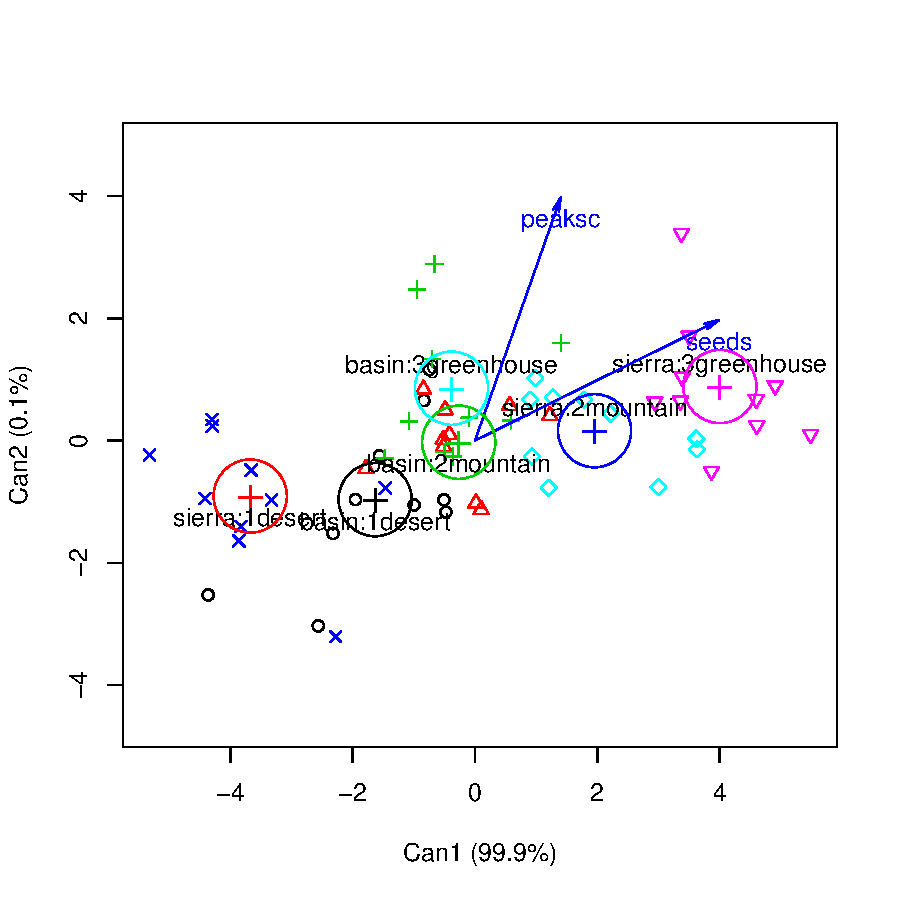
\includegraphics{HW09MANOVA_DA-007}

Based on the plot, which includes the 95 percent confidence circles for the centroids, it appears that with the potential exception of ecotype basin in locations mountain and greenhouse, all other differences are significant. These data were simulated to represent a prototypical genotype-environment interaction where a genotype specialized in an extreme environment (basin) cannot respond to improved conditions as much as one adapted to a more mesic environment.
Because there are only two response variables, there are just two canonical variables. By far, most of the differences among means are explained by Can1, the first canonical variable. According to the biplot, Can1 seems to represent mostly the variable seeds, but it is also correlated positively with peaksc.

\subsection{Exploration of the interaction [10]}

Save the Canonical 1 for the interaction. Analyze it using an lm() where Canonical 1 is the response and origin, location and origin*location are the effects. Report a plot of Canonical 1 vs. origin for each location.
\begin{Schunk}
\begin{Sinput}
> candi.ecoloc.scores <- candi.ecoloc$scores
> lm1 <- lm(Can1 ~ ecotype*location, candi.ecoloc.scores)
> summary(lm1)
\end{Sinput}
\begin{Soutput}
Call:
lm(formula = Can1 ~ ecotype * location, data = candi.ecoloc.scores)

Residuals:
    Min      1Q  Median      3Q     Max 
-2.7309 -0.6331 -0.1606  0.6769  2.2085 

Coefficients:
                                  Estimate Std. Error t value Pr(>|t|)    
(Intercept)                        -1.6334     0.3162  -5.165 3.56e-06 ***
ecotypesierra                      -2.0440     0.4472  -4.570 2.87e-05 ***
location2mountain                   1.3673     0.4472   3.057  0.00347 ** 
location3greenhouse                 1.2494     0.4472   2.794  0.00720 ** 
ecotypesierra:location2mountain     4.2657     0.6325   6.745 1.07e-08 ***
ecotypesierra:location3greenhouse   6.4332     0.6325  10.172 3.73e-14 ***
---
Signif. codes:  0 ‘***’ 0.001 ‘**’ 0.01 ‘*’ 0.05 ‘.’ 0.1 ‘ ’ 1

Residual standard error: 1 on 54 degrees of freedom
Multiple R-squared:  0.8704,	Adjusted R-squared:  0.8584 
F-statistic: 72.55 on 5 and 54 DF,  p-value: < 2.2e-16
\end{Soutput}
\begin{Sinput}
> anova(lm1)
\end{Sinput}
\begin{Soutput}
Analysis of Variance Table

Response: Can1
                 Df  Sum Sq Mean Sq F value    Pr(>F)    
ecotype           1  34.762  34.762  34.762 2.503e-07 ***
location          2 220.860 110.430 110.430 < 2.2e-16 ***
ecotype:location  2 107.135  53.567  53.567 1.515e-13 ***
Residuals        54  54.000   1.000                      
---
Signif. codes:  0 ‘***’ 0.001 ‘**’ 0.01 ‘*’ 0.05 ‘.’ 0.1 ‘ ’ 1
\end{Soutput}
\begin{Sinput}
> library(ggplot2)
> newdata <- expand.grid(ecotype=c("basin","sierra"), location =c("1desert","2mountain","3greenhouse"))
> dplot <-cbind(newdata, Can1=predict(lm1,newdata), se=predict(lm1,newdata, se.fit=TRUE)$se.fit)
> ggplot(dplot, aes(x = location, y = Can1, colour = ecotype, group=ecotype)) +
+   geom_point(aes(shape=ecotype), size=4) +
+   geom_line(aes(linetype=ecotype), size=2) +
+   geom_errorbar(aes(ymax=Can1+se, ymin=Can1-se), width=0.1)
>   labs(x = "location", y = "Predicted Can1")
\end{Sinput}
\begin{Soutput}
$x
[1] "location"

$y
[1] "Predicted Can1"

attr(,"class")
[1] "labels"
\end{Soutput}
\end{Schunk}
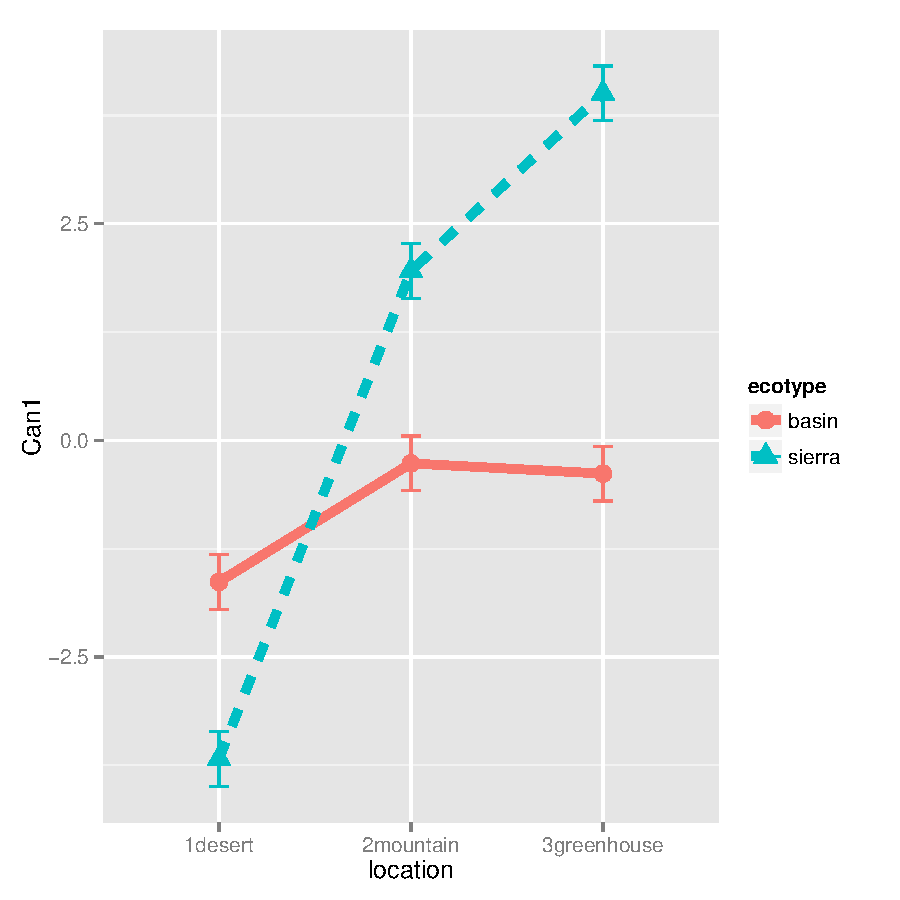
\includegraphics{HW09MANOVA_DA-008}

Note that the residual variance, estimated by the MSE of Can1 is equal to 1. This is the same for all canonical variables in MANOVA, because they are scaled such that their residual variance is 1. The plot of the canonical 1 for the interaction clearly shows the "textbook" norm of reaction of a genotype by environment interaction.

\subsection{Interpret interaction [10]}

Interpret the interaction by using the plot from the previous question and the correlations between Canonical 1 and the original response variables. These correlations tell you which variables are represented in Canonical 1 and how. Report them.

\begin{Schunk}
\begin{Sinput}
> cor(phytus[,3:4],candi.ecoloc.scores[,3:4])
\end{Sinput}
\begin{Soutput}
            Can1      Can2
seeds  0.9984281 0.4933564
peaksc 0.3508383 0.9948634
\end{Soutput}
\end{Schunk}

Canonical1 is highly correlated with seeds, and Canonical 2 is related to peaksc. However, all correlations are positive. Thus, it appears that most of the interaction effects are due to changes in the number of seeds produced. When grown in desert conditions, the basin ecotype exhibits local adaptation and produces more seeds than the sierra ecotype. In better environments, the sierra ecotype performs a lot better than basin, showing ability to exploit more humid and stable environments like the greenhouse.

\subsection{What variables appear to explain the differences?  [10]}

Use the centroid plot to determine which -if any- response variable is more responsible for the interaction effects.

The number of seeds produced seems to be the main response variable behind the multivariate differences among the treatment combinations. Again, seeds is almost perfectly aligned with the string of centroids, with the exception that the difference (not significant) between basin greenhouse and basin mountain is more related to difference in peak standing crop.




\end{document}
